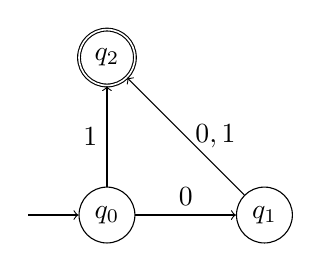
\begin{tikzpicture}
\node[draw,circle] (A) at (0,0) {$q_0$};
\draw[->] (-1,0) -- (A);
\node[draw,circle] (B) at (2,0) {$q_1$};
\node[draw,double,circle] (C) at (0,2) {$q_2$};
\draw[->] (A) -- (B);
\draw (1,0) node [above] {$0$};
\draw[->] (B) -- (C);
\draw (1,1) node [above,right] {$0,1$};
\draw[->] (A) -- (C);
\draw (0,1) node [left] {$1$};
\end{tikzpicture}